\subsection{Diseño Módulo 2}

En esta sección se establecen los fundamentos de las reglas que permiten 
clasificar automáticamente el estado del kéfir a partir de sus parámetros 
fisicoquímicos principales: pH, temperatura y concentración de $CO_{2}$. 
Con este propósito, se definen con precisión los rangos operativos de cada variable, 
junto con sus respectivas etiquetas lingüísticas y funciones de pertenencia trapezoidales, 
las cuales han sido diseñadas considerando los márgenes de error típicos de los sensores 
especificados en la sección \ref{sec:mod1}.
Por consiguiente, este enfoque transforma las mediciones crudas en información cualitativa 
robusta y significativa, creando las bases para una clasificación confiable del kéfir en 
categorías prácticas que orientan directamente la toma de decisiones del productor. 
A continuación, se describe detalladamente dicho proceso.

\subsubsection{Clasificación del kéfir}
Como primera parte para definir las clasificaciones del kéfir, 
se establecen los rangos del pH. Con base en la tabla \cref{tab:dominio_ph},
se especifican los rangos y las etiquetas lingüísticas que adopta el pH durante 
el proceso de fermentación del kéfir. Estos dominios, junto con sus respectivas 
funciones de pertenencia trapezoidales, la cual se define mediante la siguiente expresión matemática:

\begin{equation}
\mu(x) = 
\begin{cases}
0, & x \leq a \quad \vee \quad x \geq d \\[8pt]
\dfrac{x - a}{b - a}, & a \leq x \leq b \\[12pt]
1, & b \leq x \leq \\[12pt]
\dfrac{d - x}{d - c}, & c \leq x \leq d
\end{cases}
\label{eq:trapezoidal}
\end{equation}

donde \(a \leq b \leq c \leq d\) son los parámetros que delimitan el soporte y la meseta de la función.
Por lo que dicha función trapezoidal se ilustra en la \cref{fig:Log1}, 
donde se aprecia claramente la transición suave entre las categorías Óptimo, 
Adecuado, Subóptimo y Sobrefermentado.

\begin{table}[htbp]
    \centering
    \caption{Dominio de Valores de pH por Etiqueta}
    \label{tab:dominio_ph}
    \begin{tabularx}{\textwidth}{|>{\centering\arraybackslash}X|>{\centering\arraybackslash}X|>{\centering\arraybackslash}X|>{\centering\arraybackslash}X|>{\centering\arraybackslash}X|>{\centering\arraybackslash}X|}
        \hline
        \multirow{3}{*}{\textbf{Criterio}} & \multirow{3}{*}{\textbf{Etiqueta}} & \multicolumn{4}{c|}{\textbf{Dominio de pH (x)}} \\ 
        \cline{3-6} 
    
        & & \multicolumn{1}{c|}{\textbf{a $\leq$ x $\leq$ b}} & \multicolumn{2}{c|}{\textbf{b $\leq$ x $\leq$ c}} & \multicolumn{1}{c|}{\textbf{c $\leq$ x $\leq$ d}} \\ 
        \cline{3-6} 
        
        & & \textbf{a} & \textbf{b} & \textbf{c} & \textbf{d} \\ 
        \hline
        
        \multirow{5}{*}{\textbf{pH}}
        & Neutro & 6.8 & \multicolumn{3}{c|}{$\text{pH} \geq 7.0$} \\
        \cline{2-6}
        
        & Adecuado & 4.9 & 5.0 & 6.5 & 6.8 \\
        \cline{2-6} 
        
        & Semi-Ácido & 4.6 & 4.7 & 4.9 & 5.0 \\ 
        \cline{2-6} 
        
        & Ideal & 4.1 & 4.2 & 4.5 & 4.6 \\ 
        \cline{2-6} 
        
        & Muy ácido & \multicolumn{3}{c|}{$\text{pH} \leq 4.1$} & 4.2 \\ 
        \hline
    \end{tabularx}
\end{table}

\begin{figure}[htb]
    \centering
    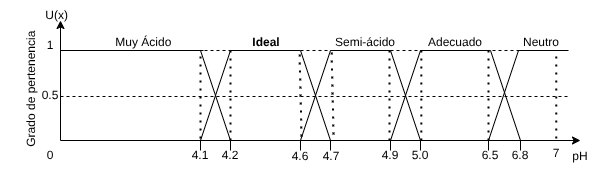
\includegraphics[width=1\textwidth]{./UML/Modulo2/diseno/logica1.drawio.png}
    \caption{Función de membresiá pH}
    \label{fig:Log1}
    \end{figure} 

De la misma manera se establecen los rangos de la temperatura y sus respectivas etiquetas 
lingüísticas en la tabla \cref{tab:dominio_temp} durante el proceso de fermentación del kéfir.
Dichos dominios siguen la misma estructura de la fórmula \eqref{eq:trapezoidal}, 
por lo que se definen las funciones de pertenencia trapezoidales en la \cref{fig:Log2}, 
donde se aprecia claramente la transición suave entre las categorías Muy baja, Baja, Normal, 
Alta y Demasiado alta.

\begin{table}[h!]
    \centering
    \caption{Dominio de Valores de Temperatura por Etiqueta}
    \label{tab:dominio_temp}
    % Se mantiene la estructura centrada y flexible de tabularx
    \begin{tabularx}{\textwidth}{|>{\centering\arraybackslash}X|>{\centering\arraybackslash}X|>{\centering\arraybackslash}X|>{\centering\arraybackslash}X|>{\centering\arraybackslash}X|>{\centering\arraybackslash}X|}
        \hline
        % Cabecera superior: Se mantiene en 3 filas de alto
        \multirow{3}{*}{\textbf{Criterio}} & \multirow{3}{*}{\textbf{Etiqueta}} & \multicolumn{4}{c|}{\textbf{Dominio de Temperatura (x)}} \\ 
        \cline{3-6} 
    
        % Los multicols deben usar 'c' o un tipo de columna centrado.
        % NOTA: Se corrige la notación de dominio a su forma común
        & & \multicolumn{1}{c|}{\textbf{a < x < b}} & \multicolumn{2}{c|}{\textbf{b < x < c}} & \multicolumn{1}{c|}{\textbf{c < x < d}} \\ 
        \cline{3-6} 
        
        & & \textbf{a} & \textbf{b} & \textbf{c} & \textbf{d} \\ 
        \hline
        
        % Se ajusta \multirow a 5 filas para contener todos los nuevos datos
        \multirow{5}{*}{\textbf{Temp.}}
        & Muy frío & $0^\circ\text{C}$ & $2^\circ\text{C}$ & $10^\circ\text{C}$ & $12^\circ\text{C}$ \\ 
        \cline{2-6} 
        
        & Frío & $10^\circ\text{C}$ & $12^\circ\text{C}$ & $16^\circ\text{C}$ & $18^\circ\text{C}$ \\ 
        \cline{2-6} 
        
        & Ambiente & $16^\circ\text{C}$ & $18^\circ\text{C}$ & $25^\circ\text{C}$ & $27^\circ\text{C}$ \\ 
        \cline{2-6} 
        
        & Caliente & $25^\circ\text{C}$ & $27^\circ\text{C}$ & $30^\circ\text{C}$ & $32^\circ\text{C}$ \\ 
        \cline{2-6} 
        
        % La última fila fusiona las columnas y se corrige la notación
        & Muy Caliente & $30^\circ\text{C}$ & \multicolumn{3}{c|}{$\text{Temp.} \geq 32^\circ\text{C}$} \\ 
        \hline
    \end{tabularx}
\end{table}

 \begin{figure}[htb]
    \centering
    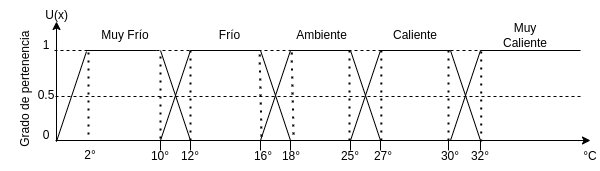
\includegraphics[width=.9\textwidth]{./UML/Modulo2/diseno/logica2.drawio.png}
    \caption{Función de membresiá Temperatura}
    \label{fig:Log2}
    \end{figure} 

\newpage 
A partir de lo anterior, se construye la matriz de reglas difusas presentada en la 
\cref{tab:reglas_ph_temp}, la cual integra las variables de entrada pH y 
temperatura para determinar la condición del kéfir en cada escenario posible para 
las 11 categorías resultantes.Las cuales se detallan exhaustivamente en la \cref{tab:condicion_kefir}, 
proporcionando al productor una guía clara para la toma de decisiones inmediata.

\begin{table}[h!]
    \centering
    \caption{Matriz de Reglas Difusas para la clasificación del kéfir.}
    \label{tab:reglas_ph_temp}
    
    % Ahora son 6 columnas
    \begin{tabularx}{\textwidth}{|X|X|X|X|X|X|}
        \hline
        
        % Fila 1
        \multirow{2}{*}{\textbf{Temp.}} & \multicolumn{5}{c|}{\textbf{pH}} \\
        \cline{2-6}
        
        % Fila 2
        & \textbf{Neutro} & \textbf{Adecuado} & \textbf{Semi-Ácido} & \textbf{Ideal} & \textbf{Muy Ácido} \\
        \hline
        
        % Filas de datos
        \textbf{Muy Frío} 
        & Inhibición (IN) 
        & Inhibición (IN) 
        & Inhibición (IN) 
        & Inhibición (IN) 
        & Riesgo Bajo (RIB) \\
        \hline
        
        \textbf{Frío} 
        & Deficiente (DEF)
        & Inicialmente Aceptable (IACE) 
        & Progresiva- mente Aceptable (PACE) 
        & Semi-Óptimo (SO) 
        & Sobreferme- ntado (SOB) \\
        \hline
        
        \textbf{Ambiente} 
        & Deficiente (DEF)
        & Inicialmente Estable (IES) 
        & Progresiva- mente Estable (PES) 
        & \textbf{Perfecto (PER)} 
        & Sobreferme- ntado (SOB) \\
        \hline
        
        \textbf{Caliente} 
        & Deficiente (DEF)
        & Inicialmente Aceptable (IACE) 
        & Progresiva- mente Aceptable (PACE) 
        & Semi-Óptimo (SO) 
        & Sobreferme- ntado (SOB) \\
        \hline
        
        \textbf{Muy Caliente} 
        & Peligro (PE)
        & Deficiente (DEF) 
        & Deficiente (DEF) 
        & Deficiente (DEF) 
        & Peligro (PE) \\ 
        \hline
    \end{tabularx}
\end{table}

\begin{table}[htbp]
    \centering
    \caption{Descripción de las clasificaciones del kéfir}
    \label{tab:condicion_kefir}
    
    \begin{tabularx}{\textwidth}{
        |>{\centering\arraybackslash}p{1.3cm}
        |>{\centering\arraybackslash}p{1.5cm}
        |>{\centering\arraybackslash}p{3cm}
        |X|}
    \hline
    \textbf{Color} & \textbf{Etiqueta} & \textbf{Nombre Completo} & \textbf{Descripción} \\
    \hline
    
    Verde & PER & Perfecto & Combinación ideal de pH y temperatura; el kéfir alcanza una acidez equilibrada y un desarrollo óptimo. \\
    \hline
    
    Azul Claro & IES & Inicialmente Estable & Condición inicial estable de pH y temperatura que favorece el desarrollo adecuado de la fermentación. \\
    \hline
    
    Azul Oscuro & PES & Progresivamente Estable & Condición estable de pH y temperatura durante la fermentación, progresando en muy buenas condiciones; requiere más tiempo para alcanzar la madurez completa. \\
    \hline  
    
    Amarillo Claro & IACE & Inicialmente Aceptable & Condición inicial aceptable de pH y temperatura para el inicio de la fermentación; no garantiza el desarrollo óptimo posterior. \\
    \hline
    
    Amarillo Oscuro & PACE & Progresivamente Aceptable & Condición aceptable durante la fermentación; no desarrolla completamente el potencial organoléptico ni probiótico. \\
    \hline
    
    Blanco & IN & Inhibición & Condición asociada a temperaturas muy bajas que inhiben el proceso; la fermentación es extremadamente lenta o se detiene. Útil solo para conservación temporal de los gránulos. \\
    \hline
    
    Marrón & SOB & Sobrefermentado & Proceso excedido por tiempo prolongado; el kéfir resulta excesivamente ácido y poco recomendable para el consumo. \\
    \hline
    
    Naranja & DEF & Deficiente & Condición dada por temperaturas extremas que generan una fermentación rápida e inadecuada; se pierde viabilidad probiótica y aumenta el riesgo de contaminación. \\
    \hline
    
    Naranja Claro & RIB & Riesgo Bajo & Condición derivada de la combinación de sobrefermentación e inhibición simultánea; representa bajo riesgo para los granos al fermentar lentamente. \\
    \hline
    
    Rojo & PE & Peligro & Situación crítica que combina sobrefermentación y altas temperaturas; puede ocasionar deterioro en los granos de kéfir. \\
    \hline
    
    Gris & SO & Semi-Óptimo & El pH alcanza el rango ideal, pero la temperatura se mantiene fuera del rango óptimo; el producto es aceptable, aunque no desarrolla plenamente su potencial organoléptico ni probiótico. \\
    \hline
    
    \end{tabularx}
\end{table}




A continuación se describen las reglas difusas obtenidas directamente de la \cref{tab:condicion_kefir}:

\begin{enumerate}

% --- Muy Frío ---
\item IF Temp. es Muy Frío AND pH es Neutro THEN Condición es Inhibición (IN)
\item IF Temp. es Muy Frío AND pH es Adecuado THEN Condición es Inhibición (IN)
\item IF Temp. es Muy Frío AND pH es Semi-Ácido THEN Condición es Inhibición (IN)
\item IF Temp. es Muy Frío AND pH es Ideal THEN Condición es Inhibición (IN)
\item IF Temp. es Muy Frío AND pH es Muy Ácido THEN Condición es Riesgo Bajo (RIB)

% --- Frío ---
\item IF Temp. es Frío AND pH es Neutro THEN Condición es Deficiente (DEF)
\item IF Temp. es Frío AND pH es Adecuado THEN Condición es Inicialmente Aceptable (IACE)
\item IF Temp. es Frío AND pH es Semi-Ácido THEN Condición es Progresivamente Aceptable (PACE)
\item IF Temp. es Frío AND pH es Ideal THEN Condición es Semi-Óptimo (SO)
\item IF Temp. es Frío AND pH es Muy Ácido THEN Condición es Sobrefermentado (SOB)

% --- Ambiente ---
\item IF Temp. es Ambiente AND pH es Neutro THEN Condición es Deficiente (DEF)
\item IF Temp. es Ambiente AND pH es Adecuado THEN Condición es Inicialmente Estable (IES)
\item IF Temp. es Ambiente AND pH es Semi-Ácido THEN Condición es Progresivamente Estable (PES)
\item IF Temp. es Ambiente AND pH es Ideal THEN Condición es Perfecto (PER)
\item IF Temp. es Ambiente AND pH es Muy Ácido THEN Condición es Sobrefermentado (SOB)

% --- Caliente ---
\item IF Temp. es Caliente AND pH es Neutro THEN Condición es Deficiente (DEF)
\item IF Temp. es Caliente AND pH es Adecuado THEN Condición es Inicialmente Aceptable (IACE)
\item IF Temp. es Caliente AND pH es Semi-Ácido THEN Condición es Progresivamente Aceptable (PACE)
\item IF Temp. es Caliente AND pH es Ideal THEN Condición es Semi-Óptimo (SO)
\item IF Temp. es Caliente AND pH es Muy Ácido THEN Condición es Sobrefermentado (SOB)

% --- Muy Caliente ---
\item IF Temp. es Muy Caliente AND pH es Neutro THEN Condición es Peligro (PE)
\item IF Temp. es Muy Caliente AND pH es Adecuado THEN Condición es Deficiente (DEF)
\item IF Temp. es Muy Caliente AND pH es Semi-Ácido THEN Condición es Deficiente (DEF)
\item IF Temp. es Muy Caliente AND pH es Ideal THEN Condición es Deficiente (DEF)
\item IF Temp. es Muy Caliente AND pH es Muy Ácido THEN Condición es Peligro (PE)

\end{enumerate}




\subsubsection{Estado de la fermentación}
Con base en el marco teórico desarrollado, la liberación de $CO_{2}$ durante la fermentación del
kéfir mantiene una relación inversamente proporcional con el pH, y este, a su vez, 
depende directamente de la temperatura, la cual ejerce un control decisivo sobre la cinética de 
ambos procesos. A mayor temperatura, el pH desciende más rápidamente, lo que provoca un aumento 
prácticamente simultáneo de los niveles de $CO_{2}$. De forma contraria, cuando la 
temperatura disminuye, la caída del pH se vuelve más lenta, lo que reduce significativamente 
la velocidad de liberación de $CO_{2}$, dado que ambos compuestos son productos del metabolismo 
conjunto de bacterias lácticas y levaduras presentes en los gránulos.
\newline
No obstante, la rapidez de esta liberación constituye un indicador crítico del estado saludable del 
cultivo. Cuando se emplea una alta concentración de gránulos en relación con un volumen reducido de leche, 
la producción de $CO_{2}$ se acelera de manera abrupta, generando condiciones de hipercarbonatación que 
comprometen el equilibrio organoléptico y la viabilidad probiótica del producto final, e incluso pueden 
derivar en sobrefermentación. Por el contrario, una proporción escasa de 
gránulos genera niveles muy bajos de $CO_{2}$, lo que, aunque no daña la salud de los microorganismos, 
prolonga considerablemente los tiempos de fermentación y retrasa la obtención de las características 
deseadas.
Por lo que se propone la clasificación por medio de un sistema difuso en cascada contemplando 
las variables de pH y temperatura, para determinar el estado del kéfir, 
y a partir de este, establecer los rangos de $CO_{2}$ que corresponden a cada estado,
ilustrada en la \cref{fig:DiagramaCascada}, donde se aprecia claramente la relación entre las variables y su impacto en la clasificación final del estado del kéfir.

\begin{figure}[htb]
    \centering
    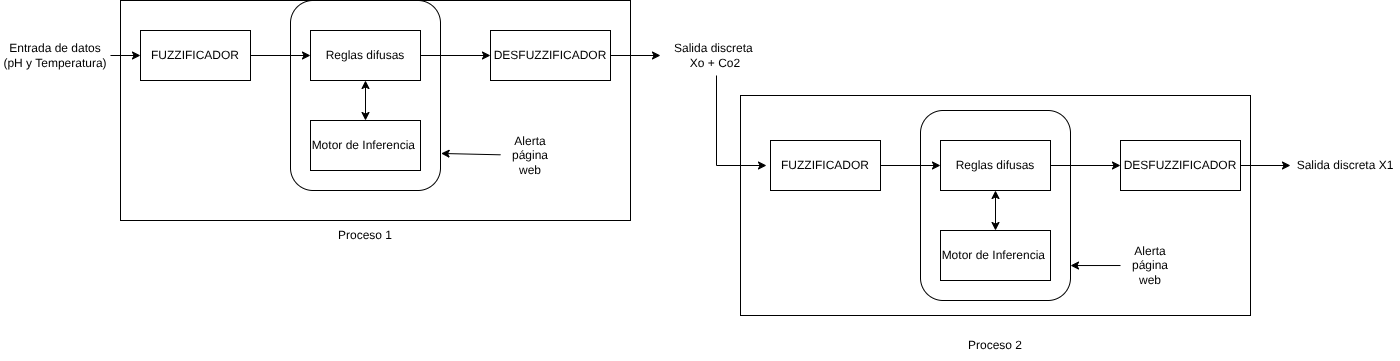
\includegraphics[width=.9\textwidth]{./UML/Modulo2/diseno/logicacascada.drawio.png}
    \caption{Diagrama de Cascada para la clasificación del estado del kéfir a partir de pH, temperatura y $CO_{2}$}
    \label{fig:DiagramaCascada}
    \end{figure} 

En consecuencia, la \cref{tab:dominio_co2} presenta los dominios difusos propuestos para la 
liberación de $CO_{2}$ durante la fermentación, estableciendo cuatro etiquetas lingüísticas Bajo, Medio, Alto y 
Excesivo expresadas en ppm, unidad entregada directamente por el sensor.

\begin{table}[htbp]
    \centering
    \caption{Dominio de Valores de $CO_{2}$ por Etiqueta}
    \label{tab:dominio_co2}

 \begin{tabularx}{\textwidth}{|>{\centering\arraybackslash}X|>{\centering\arraybackslash}X|>{\centering\arraybackslash}X|>{\centering\arraybackslash}X|>{\centering\arraybackslash}X|>{\centering\arraybackslash}X|}
        \hline
        % Cabecera superior: Se mantiene en 3 filas de alto
        \multirow{3}{*}{\textbf{Criterio}} & \multirow{3}{*}{\textbf{Etiqueta}} & \multicolumn{4}{c|}{\textbf{Dominio de CO$_2$ (ppm)}} \\ 
        \cline{3-6} 
        & & \multicolumn{1}{c|}{\textbf{a < x < b}} & \multicolumn{2}{c|}{\textbf{b < x < c}} & \multicolumn{1}{c|}{\textbf{c < x < d}} \\ 
        \cline{3-6} 

    & & \textbf{a} & \textbf{b} & \textbf{c} & \textbf{d} \\
    \hline
    \multirow{5}{*}{\textbf{CO$_2$}}
    & Muy Bajo      & 0     & 0     & 400   & 500  \\ \cline{2-6}
    & Bajo     & 400  & 500  & 1200  & 1300 \\ \cline{2-6}
    & Media     & 1200  & 1300  & 2000  & 2100  \\ \cline{2-6}
    & Alto      & 2000  & 2100  & 3200  & 3300  \\ \cline{2-6}
    & Excesivo  & 3200  &  \multicolumn{3}{c|}{$\text{$CO_{2}$} > 3300$}  \\ \hline
    \end{tabularx}
\end{table}


 \begin{figure}[htbp]
    \centering
    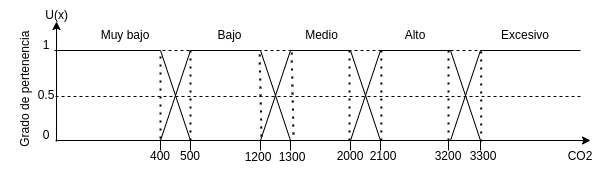
\includegraphics[width=.9\textwidth]{./UML/Modulo2/diseno/logica3.drawio.png}
    \caption{Función de membresá $CO_{2}$}
    \label{fig:Log3}
    \end{figure} 

A partir de la clasificación obtenida en la \cref{tab:condicion_kefir} 
y el dominio obtenido en la \cref{tab:dominio_co2},
podemos obenr una  nueva matriz de reglas difusas presentada en la 
\cref{tab:matriz_calidad_co2}, para determinar la salud delkéfir en 
cada escenario posible.En dnde se presentan , mismos que se describen en 
proporcionando al productor una guía sobre la salud de su kéfir.


\begin{table}[h!]
    \centering
    \caption{Matriz de Reglas Difusas para el estado del kéfir}
    \label{tab:matriz_calidad_co2}
    
    \begin{tabularx}{\textwidth}{|X|X|X|X|X|X|}
        \hline
        \multirow{2}{*}{\textbf{Condición}} & \multicolumn{5}{c|}{\textbf{Clasificación de $\text{CO}_2$}} \\
        \cline{2-6}
        & \textbf{Muy Bajo} & \textbf{Bajo} & \textbf{Medio} & \textbf{Alto} & \textbf{Excesivo} \\
        \hline
        \textbf{Perfecto (IES)} & Crítico & Satisfactorio (SA)  & Equilibrado (EQ) & Excelente (EX) & Crítico (CRI) \\
        \hline
        \textbf{Inicialmente Estable (IES)} & Equilibrado (EQ) & Equilibrado (EQ) & Malo (MA) & Malo (MA) & Crítico (CRI)\\
        \hline
        \textbf{Progresiva- mente Estable (PES)} & Malo (MA) & Equilibrado (EQ) & Satisfactorio (SA) & Malo (MA) & Crítico (CRI)\\
        \hline
        \textbf{Inicialmente Aceptable (IACE )} & Equilibrado (EQ) & Equilibrado (EQ) & Malo (MA) & Malo (MA) & Crítico (CRI) \\
        \hline
        \textbf{Progresiva- mente Aceptable (IACE)} & Malo (MA) & Equilibrado (EQ) & Satisfactorio (SA) & Malo (MA) & Crítico (CRI) \\
        \hline
        \textbf{Peligro (PE)} & Crítico (CRI) & Malo (MA)  & Malo (MA) & Equilibrado (EQ) & Crítico (CRI)  \\
        \hline
        \textbf{Semi-Óptimo (SO)} & Crítico (CRI)& Satisfactorio (SA)  & Equilibrado (EQ) & Equilibrado (EQ) &Crítico (CRI)  \\
        \hline
        \textbf{Inhibición (IN)} & Equilibrado (EQ) & Equilibrado (EQ) & Crítico (CRI)& Crítico (CRI)& Crítico (CRI)\\
        \hline
        \textbf{Sobrefer- mentado (SOB)} & Crítico (CRI)& Crítico (CRI)& Malo (MA) & Equilibrado (EQ) & Crítico (CRI)\\
        \hline
        \textbf{Deficiente (DEF)} & Crítico (CRI)& Crítico (CRI)& Equilibrado (EQ) & Equilibrado (EQ) & Crítico (CRI) \\
        \hline
        \textbf{Riesgo Bajo (RIB)} & Equilibrado (EQ) & Equilibrado (EQ) & Satisfactorio (SA) & Crítico (CRI) & Crítico (CRI)\\
        \hline
    \end{tabularx}
\end{table}

\begin{table}[htbp]
    \centering
    \caption{Descripción de las Clasificaciones del Nivel de $\text{CO}_{2}$ en la Fermentación}
    \label{tab:clasificacion_co2_mejorada}
    
    % Usamos tabularx con \textwidth y definimos el ancho de las columnas.
    % La primera columna (Color) y las dos siguientes son fijas, la última (Descripción) es flexible (X).
    \begin{tabularx}{\textwidth}{|>{\centering\arraybackslash}p{1.2cm}|c|c|X|}
    \hline
    \textbf{Color} & \textbf{Abrev.} & \textbf{Etiqueta} & \textbf{Descripción (Enfoque en la Actividad)} \\
    \hline
    \textbf{Verde} & \textbf{EX} & \textbf{Excelente} & Indica una liberación de $\text{CO}_{2}$ que corresponde a la actividad microbiana en relación con las condiciones de pH y temperatura. \\
    \hline
    \textbf{Azul} & \textbf{EQ} & \textbf{Equilibrado} & Señala una liberación de $\text{CO}_{2}$ que es la respuesta esperada de la actividad microbiana bajo las condiciones dadas de pH y temperatura, reflejando un proceso estándar. \\
    \hline
    \textbf{Ama- rillo} & \textbf{SA} & \textbf{Satisfactorio} & El nivel de $\text{CO}_{2}$ liberado es aceptable e indica una actividad microbiana funcional, aunque ligeramente por debajo de la respuesta óptima esperada para el estado de fermentación. \\
    \hline
    \textbf{Nara- nja} & \textbf{MA} & \textbf{Malo} & La liberación de $\text{CO}_{2}$ es preocupante porque no se alinea con la actividad microbiana esperada para las condiciones. Puede ser indicio de un desequilibrio en el cultivo, ya sea por un exceso de granos de kéfir en la fermentación o un contaminante externo. \\
    \hline
    \textbf{Rojo} & \textbf{CRI} & \textbf{Crítico} & Indica una liberación de $\text{CO}_{2}$ que es altamente anómala o nula en relación con el pH y la temperatura. Esto es un factor de máxima preocupación por la salud y viabilidad del cultivo. \\
    \hline
    \end{tabularx}
\end{table}

A continuación se presentan las 13 reglas difusas mínimas que reproducen exactamente la \cref{tab:matriz_calidad_co2_sinonimos_revisada}, optimizadas mediante análisis exhaustivo de patrones y uso eficiente de operadores lógicos:

\begin{enumerate}

% --- Perfecto ---
\item IF Condición es Perfecto (IES) AND CO$_2$ es Muy Bajo THEN Estado es Crítico (CRI)
\item IF Condición es Perfecto (IES) AND CO$_2$ es Bajo THEN Estado es Satisfactorio (SA)
\item IF Condición es Perfecto (IES) AND CO$_2$ es Medio THEN Estado es Equilibrado (EQ)
\item IF Condición es Perfecto (IES) AND CO$_2$ es Alto THEN Estado es Excelente (EX)
\item IF Condición es Perfecto (IES) AND CO$_2$ es Excesivo THEN Estado es Crítico (CRI)

% --- Inicialmente Estable ---
\item IF Condición es Inicialmente Estable (IES) AND CO$_2$ es Muy Bajo THEN Estado es Equilibrado (EQ)
\item IF Condición es Inicialmente Estable (IES) AND CO$_2$ es Bajo THEN Estado es Equilibrado (EQ)
\item IF Condición es Inicialmente Estable (IES) AND CO$_2$ es Medio THEN Estado es Malo (MA)
\item IF Condición es Inicialmente Estable (IES) AND CO$_2$ es Alto THEN Estado es Malo (MA)
\item IF Condición es Inicialmente Estable (IES) AND CO$_2$ es Excesivo THEN Estado es Crítico (CRI)

% --- Progresivamente Estable ---
\item IF Condición es Progresivamente Estable (PES) AND CO$_2$ es Muy Bajo THEN Estado es Malo (MA)
\item IF Condición es Progresivamente Estable (PES) AND CO$_2$ es Bajo THEN Estado es Equilibrado (EQ)
\item IF Condición es Progresivamente Estable (PES) AND CO$_2$ es Medio THEN Estado es Satisfactorio (SA)
\item IF Condición es Progresivamente Estable (PES) AND CO$_2$ es Alto THEN Estado es Malo (MA)
\item IF Condición es Progresivamente Estable (PES) AND CO$_2$ es Excesivo THEN Estado es Crítico (CRI)

% --- Inicialmente Aceptable ---
\item IF Condición es Inicialmente Aceptable (IACE) AND CO$_2$ es Muy Bajo THEN Estado es Equilibrado (EQ)
\item IF Condición es Inicialmente Aceptable (IACE) AND CO$_2$ es Bajo THEN Estado es Equilibrado (EQ)
\item IF Condición es Inicialmente Aceptable (IACE) AND CO$_2$ es Medio THEN Estado es Malo (MA)
\item IF Condición es Inicialmente Aceptable (IACE) AND CO$_2$ es Alto THEN Estado es Malo (MA)
\item IF Condición es Inicialmente Aceptable (IACE) AND CO$_2$ es Excesivo THEN Estado es Crítico (CRI)

% --- Progresivamente Aceptable ---
\item IF Condición es Progresivamente Aceptable (PACE) AND CO$_2$ es Muy Bajo THEN Estado es Malo (MA)
\item IF Condición es Progresivamente Aceptable (PACE) AND CO$_2$ es Bajo THEN Estado es Equilibrado (EQ)
\item IF Condición es Progresivamente Aceptable (PACE) AND CO$_2$ es Medio THEN Estado es Satisfactorio (SA)
\item IF Condición es Progresivamente Aceptable (PACE) AND CO$_2$ es Alto THEN Estado es Malo (MA)
\item IF Condición es Progresivamente Aceptable (PACE) AND CO$_2$ es Excesivo THEN Estado es Crítico (CRI)

% --- Peligro ---
\item IF Condición es Peligro (PE) AND CO$_2$ es Muy Bajo THEN Estado es Crítico (CRI)
\item IF Condición es Peligro (PE) AND CO$_2$ es Bajo THEN Estado es Malo (MA)
\item IF Condición es Peligro (PE) AND CO$_2$ es Medio THEN Estado es Malo (MA)
\item IF Condición es Peligro (PE) AND CO$_2$ es Alto THEN Estado es Equilibrado (EQ)
\item IF Condición es Peligro (PE) AND CO$_2$ es Excesivo THEN Estado es Crítico (CRI)

% --- Semi-Óptimo ---
\item IF Condición es Semi-Óptimo (SO) AND CO$_2$ es Muy Bajo THEN Estado es Crítico (CRI)
\item IF Condición es Semi-Óptimo (SO) AND CO$_2$ es Bajo THEN Estado es Satisfactorio (SA)
\item IF Condición es Semi-Óptimo (SO) AND CO$_2$ es Medio THEN Estado es Equilibrado (EQ)
\item IF Condición es Semi-Óptimo (SO) AND CO$_2$ es Alto THEN Estado es Equilibrado (EQ)
\item IF Condición es Semi-Óptimo (SO) AND CO$_2$ es Excesivo THEN Estado es Crítico (CRI)

% --- Inhibición ---
\item IF Condición es Inhibición (IN) AND CO$_2$ es Muy Bajo THEN Estado es Equilibrado (EQ)
\item IF Condición es Inhibición (IN) AND CO$_2$ es Bajo THEN Estado es Equilibrado (EQ)
\item IF Condición es Inhibición (IN) AND CO$_2$ es Medio THEN Estado es Crítico (CRI)
\item IF Condición es Inhibición (IN) AND CO$_2$ es Alto THEN Estado es Crítico (CRI)
\item IF Condición es Inhibición (IN) AND CO$_2$ es Excesivo THEN Estado es Crítico (CRI)

% --- Sobrefermentado ---
\item IF Condición es Sobrefermentado (SOB) AND CO$_2$ es Muy Bajo THEN Estado es Crítico (CRI)
\item IF Condición es Sobrefermentado (SOB) AND CO$_2$ es Bajo THEN Estado es Crítico (CRI)
\item IF Condición es Sobrefermentado (SOB) AND CO$_2$ es Medio THEN Estado es Malo (MA)
\item IF Condición es Sobrefermentado (SOB) AND CO$_2$ es Alto THEN Estado es Equilibrado (EQ)
\item IF Condición es Sobrefermentado (SOB) AND CO$_2$ es Excesivo THEN Estado es Crítico (CRI)

% --- Deficiente ---
\item IF Condición es Deficiente (DEF) AND CO$_2$ es Muy Bajo THEN Estado es Crítico (CRI)
\item IF Condición es Deficiente (DEF) AND CO$_2$ es Bajo THEN Estado es Crítico (CRI)
\item IF Condición es Deficiente (DEF) AND CO$_2$ es Medio THEN Estado es Equilibrado (EQ)
\item IF Condición es Deficiente (DEF) AND CO$_2$ es Alto THEN Estado es Equilibrado (EQ)
\item IF Condición es Deficiente (DEF) AND CO$_2$ es Excesivo THEN Estado es Crítico (CRI)

% --- Riesgo Bajo ---
\item IF Condición es Riesgo Bajo (RIB) AND CO$_2$ es Muy Bajo THEN Estado es Equilibrado (EQ)
\item IF Condición es Riesgo Bajo (RIB) AND CO$_2$ es Bajo THEN Estado es Equilibrado (EQ)
\item IF Condición es Riesgo Bajo (RIB) AND CO$_2$ es Medio THEN Estado es Satisfactorio (SA)
\item IF Condición es Riesgo Bajo (RIB) AND CO$_2$ es Alto THEN Estado es Crítico (CRI)
\item IF Condición es Riesgo Bajo (RIB) AND CO$_2$ es Excesivo THEN Estado es Crítico (CRI)

\end{enumerate}

\subsubsection{Segunda propuesta para la clasificación del kéfir}

Para este segundo enfoque, se propone una clasificación de manera directa,
al tomar los tres dominios de pH, temperatura y $CO_{2}$ en una matriz de 
reglas difusas misma que se describe a continuación:

% Requiere \usepackage{tabularx, multirow, ragged2e} en el preámbulo

\begin{table}[H]
    \centering
    \caption{Matriz de Reglas Difusas para la clasificación del kéfir con niveles de CO2.}
    \label{tab:reglas_ph_temp_co2}
    \begingroup
    \setlength{\tabcolsep}{3pt}
    \renewcommand{\arraystretch}{1.5}
    \footnotesize
    
    % Definimos 7 columnas: Temp + 5 de pH + 1 de CO2
    \begin{tabularx}{\textwidth}{|>{\centering\arraybackslash}p{1.6cm}|X|X|X|X|X|c|}
        \hline
        \multirow{2}{*}{\textbf{Temp.}} & \multicolumn{5}{c|}{\textbf{pH}} & \textbf{CO2} \\
        \cline{2-7}
        & \textbf{Neutro} & \textbf{Adecuado} & \textbf{Semi-Ácido} & \textbf{Ideal} & \textbf{Muy Ácido} & \textbf{Nivel} \\
        \hline
        
        \textbf{Muy Frío} & IN & IN & IN & IN & RIB & \textbf{Muy Bajo} \\ \hline
        
        \textbf{Frío} & DEF & IACE & PACE & SO & SOB & \textbf{Bajo} \\ \hline
        
        \textbf{Ambiente} & DEF & IES & PES & \textbf{PER} & SOB & \textbf{Medio} \\ \hline
        
        \textbf{Caliente} & IACE & IACE & PACE & SO & SOB & \textbf{Alto} \\ \hline
        
        \textbf{Muy Caliente} & PE & DEF & DEF & DEF & PE & \textbf{Excesivo} \\ \hline
    \end{tabularx}
    \endgroup
\end{table}

 \begin{figure}[htbp]
    \centering
    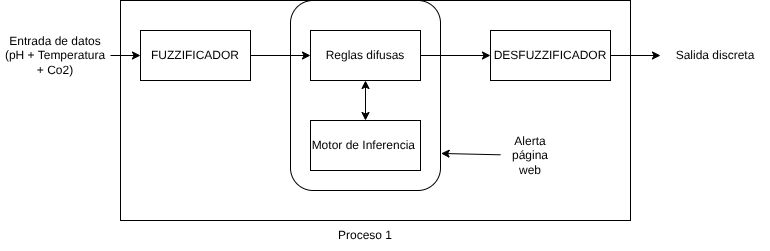
\includegraphics[width=.9\textwidth]{./UML/Modulo2/diseno/logicadiagrama.drawio.png}
    \caption{Diagrama de logica difusa a partir de pH, temperatura y Co2.}
    \label{fig:LogicaDiagrama}
    \end{figure} 

    En este ultimo enfoque se debe tomar en cuenta escenarios en las pruebas 
    más controlados, dado que se busca una clasificación directa, 
    lo que implica que cada fermentación debe realizarse en condiciones específicas 
, como por ejemplo: mantener el frasco bien cerrado para evitar la pérdida de $CO_{2}$,
 o realizar fermentaciones con cantidades de gránulos y leche estandarizadas para controlar 
 la producción de $CO_{2}$, 
 entre otros factores que podrían afectar la precisión de la clasificación.